\section{Machine learning}

\subsection{Environment}

In addition to the previous section's list of tools and libraries, we can mention \texttt{scikit-learn} whose SVM's implementation we use for our experiments. We also use its utility functions for data splitting and for metrics.

To define and train our neural networks, we use \texttt{keras} with \texttt{tensorflow} as the backend.

On our computing server, equipped with an NVidia GTX1070 graphics card, we use \texttt{tensorflow-gpu} to accelerate the calculations by using said graphics card.

% -------------------------------------------------------------------------------------------------------------
\subsection{Model architectures}

For all of the models described hereafter, we have made the input dimensions and the number of outputs modular. The goal is to be able to build different experiments easily and compare performance.

First, we use the Support Vector Machine (SVM) model provided by \texttt{sklearn} as a "control experiment". If the SVM's performance is as good or better than our more advanced models, we can worry that something is wrong. Either the problem is too easy, which probably means there are biases in the dataset, or our other models are not appropriate for the task.

Our first attempt at a Convolutional Neural Network (CNN) is based on the description in the work of \textcite{riyaz_deep_2018}. A representation of the layers is shown in figure \ref{fig:cnn-riyaz}. It achieved reasonable performance but was very prone to overfitting. Despite adding l2 regularization and increasing the dropout rate, this model still showed significant overfitting.

We later discovered that this was linked to the layer on which we performed the dropout operation. Indeed, it seems that in this situation, dropping out after the pooling layer, as opposed to doing it after the convolution layer, is a lot more effective. At this point, we had already started using the next CNN, which gave us slightly better results.

\begin{figure}[htbp!]
  \centering
  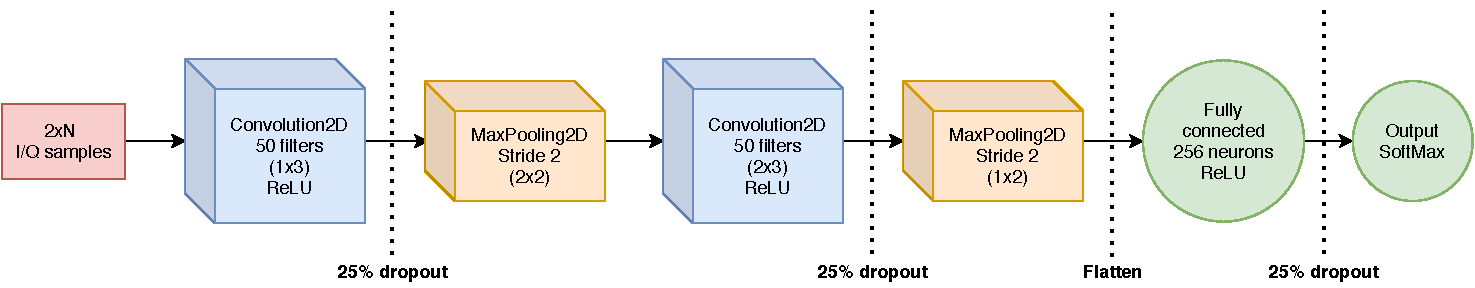
\includegraphics[scale=0.63]{figures/ml_riyaz.pdf}
  \caption{Representation of the first CNN used}
  \label{fig:cnn-riyaz}
\end{figure}

Said CNN is based on \textcite{youssef_machine_2017}'s description of their model. It is very similar to the previous one, but the convolution parameter seem more sensible and gave better results in our case. A representation of the model's layers is shown in figure \ref{fig:cnn-youssef}.

We tried adding an additional convolution layer to improve our accuracy but the performance boost was insignificant and of course it made the model slower to converge. The same applied when adding an additional dense layer. Increasing the number of neurons in the dense layer had a similar effect and also seemed to increase overfitting.

So it seems like this simple model is hard to improve upon. In the end, we added the dropout effect to the dense layer in addition to the pooling layers, in order to lower the tendency to overfit even more.

\begin{figure}[htbp!]
  \centering
  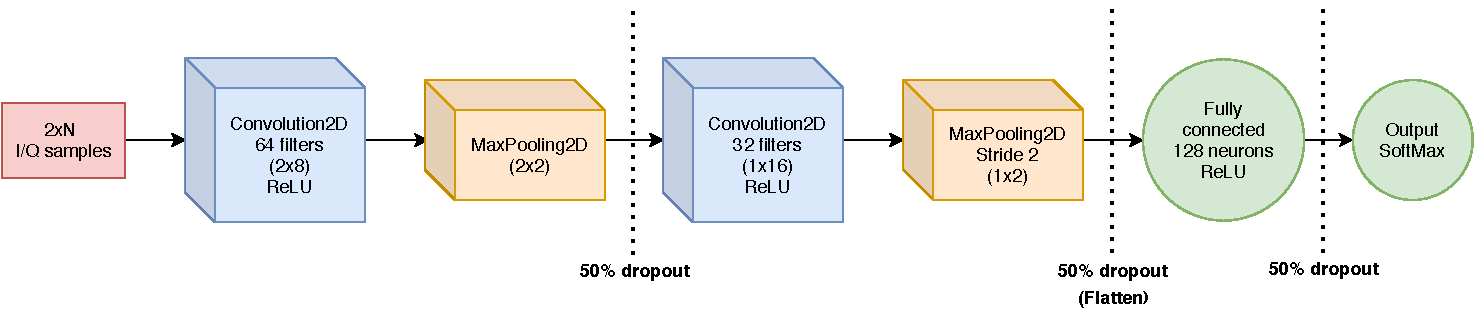
\includegraphics[scale=0.63]{figures/ml_youssef.pdf}
  \caption{Representation of the second CNN used}
  \label{fig:cnn-youssef}
\end{figure}

% -------------------------------------------------------------------------------------------------------------
\subsection{Default parameters}

Except if stated otherwise, the following experiments will use the model parameters listed in table \ref{tab:parameters}.

\begin{table}[htbp!]
  \centering
  \begin{tabular}{|l|l|}
    \hline
    \textbf{Parameter}             & \textbf{Value}            \\ \hline \hline
    \textbf{Window size}           & 512                       \\ \hline
    \textbf{Optimizer}             & Adam                      \\ \hline
    \textbf{Initial learning rate} & 0.001                     \\ \hline
    \textbf{Loss function}         & Categorical cross entropy \\ \hline
    \textbf{Batch size}            & 500                       \\ \hline
    \textbf{Number of epochs}      & 200                       \\ \hline
  \end{tabular}
  \caption{Default model parameters for our experiences}
  \label{tab:parameters}
\end{table}

% -------------------------------------------------------------------------------------------------------------
\subsection{Documenting experiments}

\subsubsection{Discriminating between chip types}

The first experiment we report on is about classifying tags from different types. To do so, we use tags 1, 6 and 9 from the first dataset. The first is an NTAG213, the second a MiFare 1k and the last a FeliCa chip. As the first dataset is quite small, we use it in its entirety, rather than applying the peak detection algorithm on it. Our SVM attained an accuracy of 69\%, and the confusion matrix is shown in figure \ref{fig:cmsvmchip}.

\begin{figure}[htbp!]
  \centering
  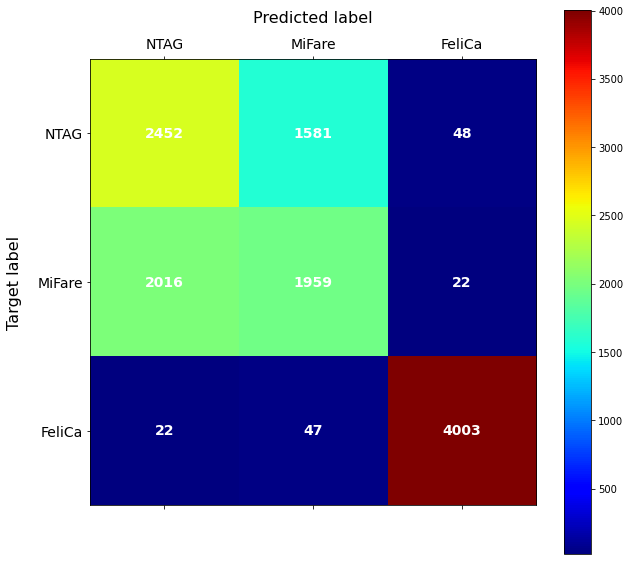
\includegraphics[scale=0.5]{figures/ml_svmchip512.png}
  \caption{Confusion matrix for the first experiment on SVM}
  \label{fig:cmsvmchip}
\end{figure}

At this task, our CNN performed slightly better with an accuracy of 74\%. Its confusion matrix is shown in figure \ref{fig:cmcnnchip}.

\begin{figure}[htbp!]
  \centering
  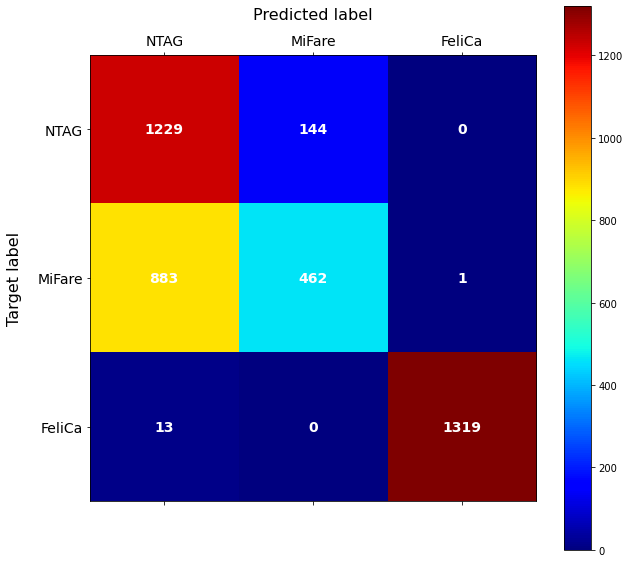
\includegraphics[scale=0.5]{figures/ml_cnnchip512.png}
  \caption{Confusion matrix for the first experiment on CNN}
  \label{fig:cmcnnchip}
\end{figure}

As we had anticipated, discriminating between our NFC-A tags (the NTAG and the MiFare) and the FeliCa tag is trivial, but finding the difference between NFC-A tags is a lot more difficult. Here the SVM probably does little better than random guessing for the first two classes.

This experience is what motivated us not to include the FeliCa tag in the second dataset. It shows that its presence doesn't add any value to the experiments.

\subsubsection{Discriminating between tags}

Here, we use the second dataset with the peak finding algorithm to evaluate the performance of our model in the scenario that interests us the most: discriminating between individual tags. Is our model able to extract features to fingerprint the devices?

In figure \ref{fig:svmcnn}, we compare the accuracy of our model for different number of tags with the accuracy of the SVM for the same numbers of tags. Of course, such a simple summary doesn't capture the full picture, but it gives a good idea of the performance of each model in different conditions. We ran the training several times and confirm that those scores are consistent.

\begin{figure}[htbp!]
  \centering
  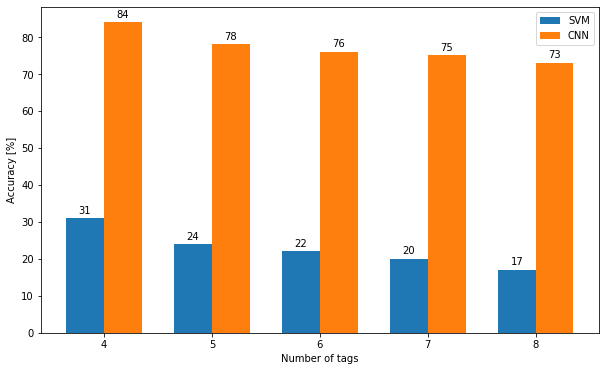
\includegraphics[scale=0.65]{figures/ml_svmcnn.png}
  \caption{SVM and CNN accuracy per number of tag}
  \label{fig:svmcnn}
\end{figure}

We'll now observe the performance of our CNN when trying to discriminate between our eight tags. For this experiment, we increased the window size to 640, and found that it consistently gave slightly better results in this scenario. Continuing to increase the window size past this number does not help the performance.

In this experiment, we got an accuracy of 76\%. The confusion matrix is detailed in figure \ref{fig:cnn640} and we can see how close together the training accuracy and the validation accuracy are in figure \ref{fig:cnn640acc}. This indicates a welcome lack of overfitting with these parameters.

\begin{figure}[htbp!]
  \centering
  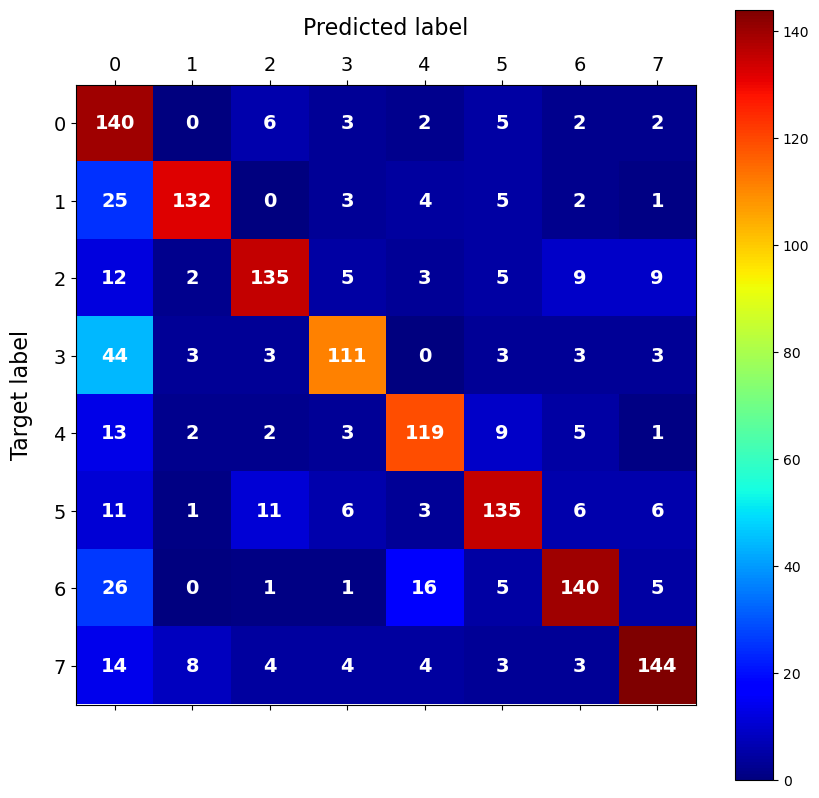
\includegraphics[scale=0.6]{figures/ml_cnn640cm.png}
  \caption{Confusion matrix for the CNN experiment}
  \label{fig:cnn640}
\end{figure}

\begin{figure}[htbp!]
  \centering
  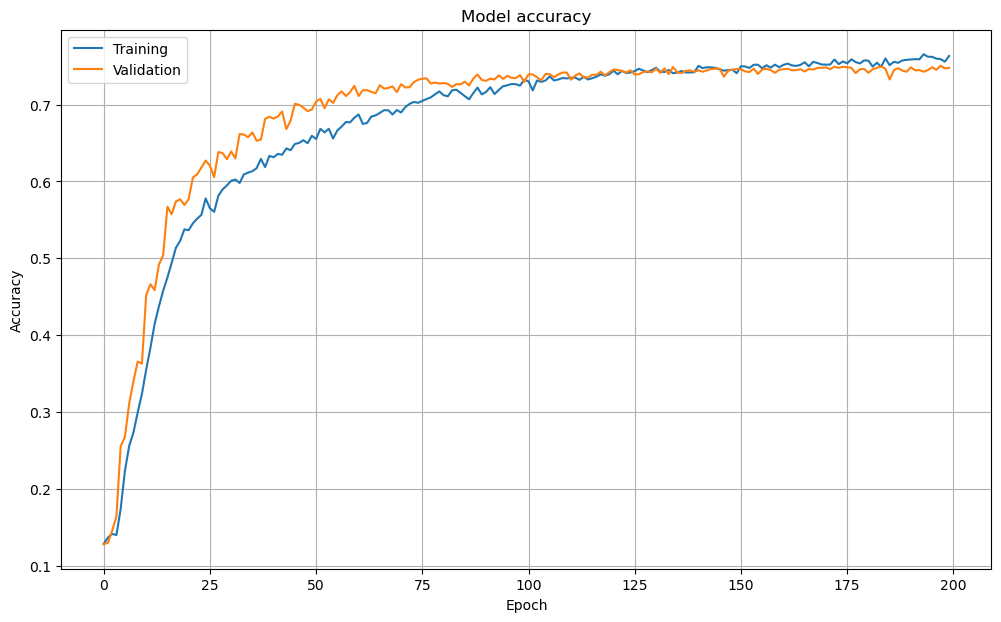
\includegraphics[scale=0.6]{figures/ml_cnn640acc.png}
  \caption{Accuracy history for the CNN experiment}
  \label{fig:cnn640acc}
\end{figure}

\begin{figure}[htbp!]
  \centering
  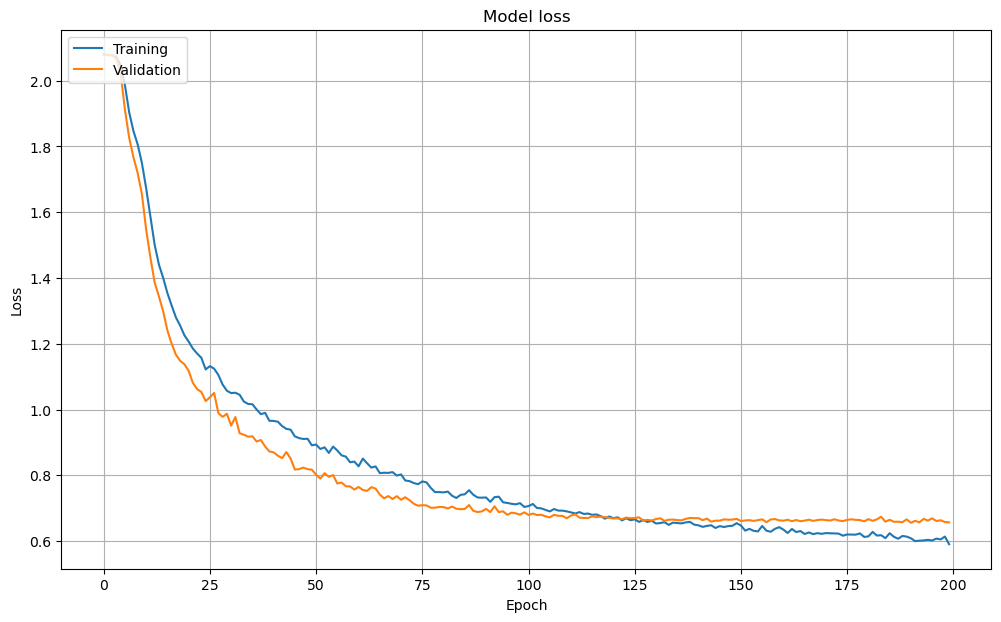
\includegraphics[scale=0.6]{figures/ml_cnn640loss.png}
  \caption{Loss history for the CNN experiment}
  \label{fig:cnn640loss}
\end{figure}

We also observed the model after 500 epochs to make sure it didn't continue to improve after the 200 standard epochs. This is not the case as the validation accuracy locks at around 75\% accuracy, while the model starts to overfit slightly.

% -------------------------------------------------------------------------------------------------------------
\subsection{Thoughts on the results}

76\% top accuracy is not a very high number, but it is high enough to prove the network is able to extract features which belong to an individual tag. On the other hand, it is not so high as to show that the problem is trivial, or that we have made it trivial by mishandling some element of the pipeline.

The fact that the SVM performs barely 5\% better than a random guess ($1/8 = 0.125$) in the most complicated scenario shows that the problem is hard. Any bias we could have introduced in the acquisition phase doesn't seem to make the problem easier. Despite this, our CNN is able to solve the problem, at least to some extent.

Furthermore, all the confusion matrices and accuracy scores we have shown here come from the trained model making prediction on the testing set. It has never seen those specific signal windows during training, which is another indicator that the features extracted by the convolution layers are meaningful.

Finally, as we could see from figures \ref{fig:cnn640acc} and \ref{fig:cnn640loss}, our CNN with these parameters isn't really prone to overfitting. The validation accuracy doesn't stay down while the training accuracy increases, as was the case with the first CNN we used. One last positive indicator is the stability of the accuracy and the loss. There is no rough movement up and down, which means the adam optimizer is able to do its job without trouble.

All these points tend to show that we met our goal, at least in some proportion. However, the numbers tell us that this is not a scalable solution. Figure \ref{fig:svmcnn} clearly shows how quickly the accuracy drops as the number of devices increases. This is consistent with the findings of some of the papers we considered for this thesis. This is why we mentioned alternative ways or additional steps in the pipeline at several points in this report. It is important to go further and inspect additional techniques to refine the process in the future. This field is very new and very active at the time of writing, exciting evolutions will happen.
